\documentclass[a4paper]{article}
\usepackage[utf8]{inputenc}
\usepackage{amsmath}
\usepackage{amsfonts}
\usepackage{amssymb}
\usepackage{graphicx}
\usepackage{flexisym}
\usepackage{geometry}
\setlength{\voffset}{-0.75in}
\setlength{\textheight}{700px}
\begin{document}

\title{
Physics \\
\large Semester 1 2017
}
\author{Cxo05}

\maketitle

\section{Simple Harmonic Motion}
Simple harmonic motion is the motion of an object whose restoring force is directly proportional to its displacement.

\begin{center}
Angular Frequency $\omega = 2\pi f$
\end{center}

\begin{center}
$f = \displaystyle\frac{1}{T}$
\end{center}

\subsection{Horizontal Spring Mass System}
\begin{center}
$F_{x} = -kx$
\end{center}

\begin{center}
$F = ma$
\end{center}

\begin{center}
$ma = -kx$
\end{center}

\begin{center}
$
a = \displaystyle\frac{F_{x}}{m} = -\frac{k}{m}x
$
\end{center}

\subsection{Energy in Simple Harmonic Motion}
We know that the object has both kinetic energy and potential energy from the spring.
\begin{center}
$K.E. = \displaystyle\frac{1}{2} mv_{x}^{2}$ and $P.E. = \displaystyle\frac{1}{2}kx^{2}$
\end{center}
Since energy is conserved, we combine the two equations.
\begin{center}
$T.E. = \displaystyle\frac{1}{2} mv_{x}^{2} + \frac{1}{2}kx^{2}$
\end{center}
Solving for $v_{x}$,
\begin{center}
$v_{x} = \displaystyle \pm\sqrt{\frac{k}{m}}\sqrt{A^{2}-x^{2}} = \omega\sqrt{A^{2}-x^{2}}$
\end{center}
Maximum velocity occurs at $x = 0$,
\begin{center}
$v_{max} = \displaystyle \sqrt{\frac{k}{m}}A$
\end{center}
\subsection{Vertical Oscillations}
When a mass is hung on an unstretched vertical spring with spring constant $k$, the string extends by $\Delta L$.
\begin{center}
$k\Delta L = mg$
\end{center}
For springs in parallel,
\begin{center}
$k_T = k_1 + k_2$
\end{center}
For springs in series,
\begin{center}
$\displaystyle k_T = \left(\frac{1}{k_1}+\frac{1}{k_2}\right)^{-1}$
\end{center}
\subsection{Circle of Reference}
\begin{center}
  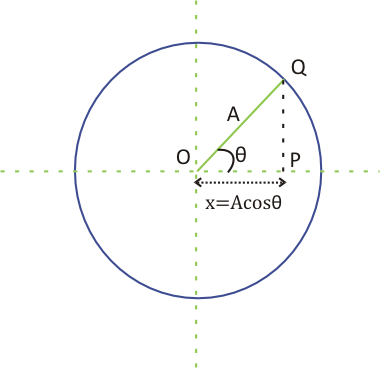
\includegraphics[width=5 cm]{CircleOfReference.png}
\end{center}
Point Q of moves in a counter clockwise direction. The constant angular velocity of Q is equals to the angular frequency of $P$'s SHM.
\begin{center}
$\omega = \Delta\phi/\Delta t$
\end{center}
From the figure, we can see that $x = A\cos{\theta}$. Note that $\phi = \theta$.
If Q is at the extreme right end of the diameter at $t = 0$, then $\phi = 0$.
\begin{center}
$\phi = \omega t$
\end{center}

\begin{center}
$x = A\cos{\omega t}$
\end{center}
The velocity of $Q$ is obtained by taking the derivative of  $x = A\cos{\omega t}$ with respect to $t$.     
\begin{center}
$v_{x} = -\omega A\sin{\omega t}$
\end{center}
     
\begin{center}
$a_{Q} = \omega^{2} A$
\end{center}

\begin{center}
$a_{x} = -\omega^{2} A\cos{\omega t}$
\end{center}
Combining the above and $x = A\cos{\omega t}$,
\begin{center}
$a_{x} = -\omega^{2}x$
\end{center}
We are now able to express the frequency of an object with respect to $k$ and $m$.
\begin{center}
$\omega^{2} = \displaystyle\frac{k}{m}$
\end{center}
\begin{center}
$f = \displaystyle\frac{1}{2\pi}\sqrt{\frac{k}{m}}$
\end{center}
\begin{center}
$T = 2\pi\sqrt{\displaystyle\frac{m}{k}}$
\end{center}
We are hence able to simplify some equations.  
\begin{center}
$a_{x} = -\displaystyle\frac{k}{m} x$
\end{center}
\begin{center}
$v_{x} = \displaystyle\pm\omega\sqrt{A^{2}-x^{2}}$
\end{center}
\textbf{IMPORTANT} When $x_{0} \ne A$, $x = A\cos{(\omega t+\phi_{0})}$, where $\phi_{0}$ is the phase constant, found by setting $t = 0$. 
\subsection{The simple pendulum}
The restoring force of a pendulum is the component of force tangent to the circular path at that point.
\begin{center}
$F = -mg\sin{\theta}$
\end{center}
With small angle approximation however, $\sin{\theta}$ is almost equals to $\theta$ in radians.
\begin{center}
$ \displaystyle F = -mg\theta = -mg\frac{x}{L}$
\end{center}
The constant $mg/L$ thus represents the force constant $k$.
\begin{center}
$\omega = \displaystyle\sqrt{\frac{k}{m}} = \sqrt{\frac{g}{L}}$
\end{center}
\subsection{Damped and forced oscillations}
Damping causes a decrease in amplitude. An additional force acting on the object that varies with time in a period way is a driving force. 

\section{Waves}
There are two types, transverse and longitudinal waves and can be represented by snapshot graphs and history graphs.
\newline 
Snapshot graphs follows all particles at one single time, $\Delta y , x$.
\newline
History graphs follows only one particle but at all times, $\Delta y, t$.
\subsection{Periodic mechanical waves}
The very important formula,
\begin{center}
$v = \lambda f$
\end{center}
Each wave advances by one wavelength $\lambda$ during each period $T$. Particles one wavelength apart move in phase with each other. 
\subsection{Wave speeds}
The speed of a transverse wave in a rope under tension is proportional to the square root of the tension, divided by the mass per unit length.
\begin{center}
$v = \displaystyle\sqrt{\frac{F_{T}}{\mu}}$
\end{center}
\subsection{Mathematical description of a wave}
Suppose that the displacement of a particle at the left end at $x = 0$.
\begin{center}
$y = A\sin{\omega t}$
\end{center}
The wave travels from $x = 0$ to some point $x$ to the right of the origin in an amount of time given by $x/v$, where $v$ is the wave speed. So the motion of point $x$ at time $t$ is the same as the motion of point $x = 0$ at the earlier time $(t - x/c)$. 
\begin{center}
$y(x,t) = \displaystyle A\sin{\omega \left(t-\frac{x}{v}\right)}$
\end{center}
\begin{center}
$y(x,t) = \displaystyle A\sin{\omega \left(\frac{t}{T}-\frac{x}{\lambda}\right)}$
\end{center}
Thus at $x = 0$,
\begin{center}
$y = \displaystyle A\sin{2\pi\frac{t}{T}}$
\end{center}
Wave number k.
\begin{center}
$k = \displaystyle\frac{2\pi}{\lambda}$
\end{center}
Phase difference $\phi_0$ in waves.
\begin{center}
$\displaystyle\frac{\Delta\phi}{2\pi} = \frac{\Delta x}{\lambda}$
\end{center}
When the particle is moving in the positive x direction, $kx-\omega t$ and in negative x direction, $kx+\omega t$.
\begin{center}
$y(x,t) = \displaystyle A\sin{(kx-\omega t + \phi_0)}$
\end{center}
\subsection{Reflections and superposition}
\subsubsection{Wave reflection}
Waves reflecting on a fixed end. When the pulse arrives, the rope exerts an upward force on the wall and the wall exerts a downward force on the rope. The pulse thus inverts as it reflects. \newline
Waves reflecting on a free end. When the pulse arrives, no force acts on the wave, thus, it reflects without inverting.
\subsubsection{Wave overlap}
When pulses overlap, the displacement of the string at any point is the vector sum of the displacements due to the individual pulses. 
\subsection{Standing waves and normal modes}
\subsubsection{Standing waves}
Nodes, points on the wave that do not move.
Anti-nodes, points midway between nodes, with the greatest amplitude. Because it does not seem to move along the string, it is called a standing wave.
\newline
Open ends of a pipe is always a displacement anti-node. Closed end of a pipe is always a displacement node.
\subsubsection{Normal modes}
Wavelengths for standing waves in strings/Closed-Closed tubes/Open-Open tubes. Largest wavelength is when $m_{mode} = 1$ and only has one anti-node.
\begin{center}
$NN = \displaystyle\frac{\lambda_{m}}{2} = \frac{L}{m}$
\end{center}
\begin{center}
$f_1 = \displaystyle\frac{v}{2L}$
\end{center}
\begin{center}
$f_m = \displaystyle m\frac{v}{2L}$
\end{center}
$m = 1$ Fundamental frequency
\newline
$m = 2$ Second Harmonic, First overtone
\newline
$...$
\newline
For Open-Close tubes however, the fundamental mode has only one quarter of a wavelength in a tube of length $L$, hence the $m = 1$ wavelength is $\lambda_1 = 4L$.
\begin{center}
$AN = \displaystyle\frac{\lambda_m}{4} = \frac{L}{m}$
\end{center}
\begin{center}
$f_m = \displaystyle m\frac{v}{4L} = mf_1$
\end{center}
\begin{center}
Where m = 1,3,5,7 \ldots
\end{center}
Fundamental frequency on a vibrating string.
\begin{center}
$f_1 = \displaystyle\frac{1}{2L}\sqrt{\frac{F_T}{\mu}}$
\end{center}

\subsection{Beats}
If two waves at first are in phase, they will interfere constructively and a large amplitude resultant wave occurs. When the two waves move, they become progressively out of phase until they interfere destructively and a low amplitude resultant wave occurs. 
\subsection{The Doppler effect}
When a source of sound is moving away from the receiver, it has a lower apparent frequency. When a source of sound is moving towards the receiver, it has a high apparent frequency.  
\subsection{Power and Intensity of wave}
If a wave has power $P$,
\begin{center}
$I = \displaystyle\frac{P}{Area}$
\end{center}
If a source of spherical waves radiates uniformly in all directions,
\begin{center}
$I = \displaystyle\frac{P_{source}}{4\pi r^2}$
\end{center}
\begin{center}
$\displaystyle \frac{I_1}{I_2} = \frac{{r_2}^2}{{r_1}^2}$
\end{center}
\section{Lens}
Image is always virtual when outgoing rays don't actually come from the image.
\begin{itemize}
\item When object on same side as reflecting surface, distance is positive.
\item When image is on same side as reflecting surface, the distance is positive.
\end{itemize}
\subsection{Plane mirrors}
Object and image will have the same size and orientation when using plane mirrors.
\begin{center}
$s = -s\textprime$
\end{center}
Image formed is always upright but reversed.

\subsection{Reflections at a spherical surface}
\begin{center}
  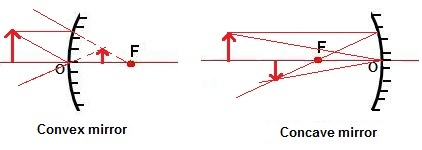
\includegraphics[width=10 cm]{curvedmirrors.jpeg}
\end{center}
$F$ is the focal point. Center of curvature $C$ is between $F$ and $2F$. $R$ is the distance between $C$ and the surface. $f$ is the distance between $F$ and the surface.
\subsubsection{Focal length}
\begin{center}
$\displaystyle \frac{1}{s} + \frac{1}{s\textprime} = \frac{2}{R} = \frac{1}{f}$
\end{center}
When $C$ is on the same side as the outgoing ray, $R$ is positive.
\subsubsection{Lateral magnification}
\begin{center}
$m = \displaystyle\frac{y\textprime}{y} = -\frac{s\textprime}{s}$
\end{center}
\textbf{IMPORTANT} Both equations can be used for both concave and convex mirrors and lens. 
\subsubsection{Drawing ray diagrams}
\begin{center}
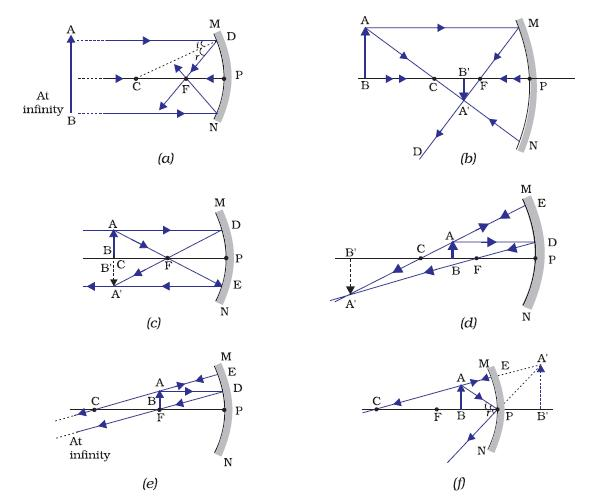
\includegraphics[width=9 cm]{drawing_rays.jpg}
\end{center}
\subsection{Refraction}
\begin{center}
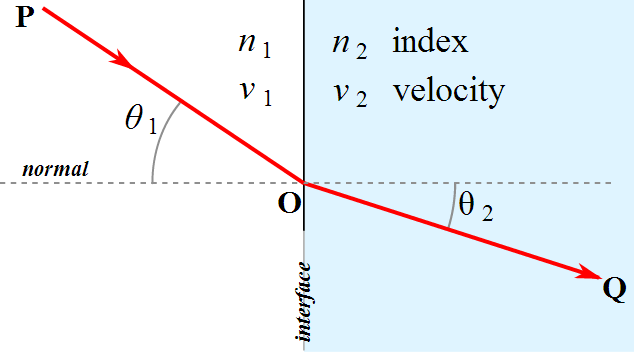
\includegraphics[width=7 cm]{refraction.png}
\end{center}
\begin{center}
$n_1sin\theta_1 = n_2sin\theta_2$
\end{center}
Total internal reflection occurs when the angle of incidence is more than or equals to critical angle. To find critical angle, we use Snell's law.
\begin{center}
$\displaystyle\theta_c = sin^{-1}\left(\frac{n_2}{n_1}\right)$
\end{center}
\subsubsection{Refraction at a spherical surface}
\begin{center}
$\displaystyle\frac{n_a}{s} + \frac{n_b}{s\textprime} = \frac{n_b - n_a}{R}$
\end{center}
\begin{center}
$m = \displaystyle\frac{n_as\textprime}{n_bs}$
\end{center}
At a plane surface where $R = \infty$.
\begin{center}
$\displaystyle\frac{n_a}{s} + \frac{n_b}{s\textprime} = 0$
\end{center}
\subsection{Thin lens}
Equation for focal length and lateral magnification can be applied.
\newline
\textbf{IMPORTANT} When half the lens is covered, the image is blurred.
\subsubsection{Lens-maker equation}
\begin{center}
$\displaystyle \frac{1}{s} + \frac{1}{s\textprime} = \frac{2}{R} = \frac{1}{f} = (n - 1)\left(\frac{1}{R_1}-\frac{1}{R_2}\right)$
\end{center}
\begin{center}
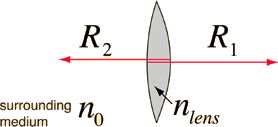
\includegraphics[width=6 cm]{lenmaker.png}
\end{center}
Sign conventions for $R$:
\begin{itemize}
\item $+/-$ for both sides convex
\item $+/+$ for left side convex, right side concave
\item $-/+$ for both sides concave
\item $-/-$ for left side concave, right side convex
\end{itemize}
\subsection{Multiple lens}
When two lens are placed right next to each other, in contact.
\begin{center}
$\displaystyle\frac{1}{F} = \frac{1}{f_1} + \frac{1}{f_2}$
\end{center}
\subsubsection{Microscope}
A microscope consists of two lens, the eyepiece with the angular magnification $M_2$ and the objective with lateral magnification $m_1$.
\begin{center}
$\displaystyle M = m_1M_2 = \frac{(25cm)(D_{i objective})}{f_1f_2}$
\end{center}
\subsubsection{Telescope}
The telescope works in a similar way like the microscope.
\begin{center}
$M = \displaystyle-\frac{f_1}{f_2}$
\end{center}
Where $f_1$ is eyepiece and $f_2$ is objective.
\begin{center}
\vfill
\fbox{
This thus concludes the summary for Year 4 Physics Semester 1 2017.
}
\end{center}
\end{document}
